\documentclass[unknownkeysallowed]{beamer}
\usepackage[utf8]{inputenc}
\usepackage[T1]{fontenc}
\usepackage{mathabx}
\usepackage{mathpazo}
\usepackage{eulervm}
\usepackage{natbib}

%% Load the markdown package
\usepackage[citations,footnotes,definitionLists,hashEnumerators,smartEllipses,tightLists=false,pipeTables,tableCaptions,hybrid]{markdown}
%%begin novalidate
\markdownSetup{rendererPrototypes={
 link = {\href{#2}{#1}},
 headingOne = {\section{#1}},
 headingTwo = {\subsection{#1}},
 headingThree = {\begin{frame}\frametitle{#1}},
 headingFour = {\begin{block}{#1}},
 horizontalRule = {\end{block}}
}}
%%end novalidate

\usetheme{Copenhagen}
\usefonttheme{serif}
\usecolortheme{dove}

\usebackgroundtemplate 
{
\includegraphics[width=\paperwidth]{figuras/bkg.jpg}}
\addtobeamertemplate{title page}{}{\begin{center}Orientar: Adson Rocha\end{center}}

\title[Processamento do EMG com ML e Entropia]{Electromyographic Signal Processing Using Machine Learning and Entropy}
\author{Luiz Barbosa}
\institute{Universidade de Brasília}

\setbeamertemplate{headline}{}
\addtobeamertemplate{headline}{}
{
    \leavevmode%
    \hbox{%
    \begin{beamercolorbox}[wd=.4\paperwidth,ht=3.5pc]{}
        \begin{figure}
            
\includegraphics[height=1cm,width=1cm,keepaspectratio]{figuras/logo2.png}
            \hspace{0.2cm}
            
\includegraphics[height=0.9cm,width=0.9cm,keepaspectratio]{figuras/logo4.png}
        \end{figure}
    \end{beamercolorbox}%
    \begin{beamercolorbox}[wd=.3\paperwidth,respectlinebreaks,center]{}
        Universidade de Brasília - UnB \\
        Faculdade UnB Gama - FGA \\
        Mestrado em Engenharia Biomédica
        \vspace{\floatsep}
    \end{beamercolorbox}%
    \begin{beamercolorbox}[wd=.3\paperwidth,ht=3.5pc]{}
        \begin{figure}
            
\includegraphics[height=1cm,width=1cm,keepaspectratio,left]{figuras/logo3.png}
        \end{figure}
    \end{beamercolorbox}}%
    \vskip0pt%
}

{ 

\begin{document}

\maketitle

\frame{\tableofcontents}

\begin{markdown}
%%begin novalidate

# Introdução

%### Ref. provisória
%
%- Yeah to some extent, with \texttt{markdown} package :-)
%    - __$\hash$__ and __$\hash\hash$__ for section and subsection headers (in ToC)
%    - Redefine __$\hash\hash\hash$__ to start a frame and frametitle
%    - (Nested) bullet and numbered lists
%    - Text formatting (*italic*, **bold becomes italic + alerted**) 
%    - Redefine __$\hash\hash\hash\hash$__ to start a block with title \linebreak
%      and __\texttt{-{}-{}-{}-}__ to end the block
%    - ___Compile with \texttt{-{}-shell-escape}___ (Overleaf does this already)
%- (Alternative approaches: Pandoc, wikitobeamer)
%
%\end{frame}
%
%%%%%%%%%%%%%%%%%%%%%%%
%
%### Caveats
%
%- Nothing too complicated! 
%- No verbatim or fragile stuff!
%- No $\hash$ and \textunderscore{} characters!\linebreak 
%  (I used `$\hash$` and `\textunderscore`)
%- Can't pass options to frames
%- __Need to write \texttt{\textbackslash end\string{frame\string}} manually!__
%
%\end{frame}
%
%%%%%%%%%%%%%%%%%%%%%%%
%
%### Projected Profit
%
%1. And the answer is...
%2. $f(x)=\sum_{n=0}^\infty\frac{f^{(n)}(a)}{n!}(x-a)^n$
%    #. How do we _know_ that?
%    #. __Maths!__
%
%\end{frame}

%%%%%%%%%%%

%- This is a citation [@novotny:2017]
%- Works like `natbib` syntax [see @novotny:2019 p.26]

%\end{frame}

%%%%%%%%%%%

## Problemática
### O Sinal sEMG

- Variabilidade do sinal sEMG:
    - O sinal EMG varia de acordo com a postura, posição e força aplicada pela pessoa que está realizando uma contração muscular.
    - Próteses têm um investimento de alto custo, muitas vezes não é possível oferecer treinamento a longo prazo para seu uso.
    - Processamento em tempo real exige janelas temporais muito pequenas, o que limita a informação extraída do sinal e a classificação do mesmo. 
    - Crescente complexidade das redes neurais utilizadas para a classificação do sinal.

\end{frame}

%%%%%%%%%%%%%%%%%%%%%%

### Datasets

- Dificuldade de datasets:
    - Os  dados  do  sinal  EMG  são  adquiridos  em  um  curto período  de  duração,  os parâmetros coletados contêm informações limitada.
    - Ampliar o tempo de coleta de dados se torna impraticável, pois adicionaria uma carga muito grande ao usuário. 
    - Os sistemas de próteses que utilizam controle de reconhecimento de padrões mio-elétricos não são comercializados por possuírem desempenho insatisfatório.

\end{frame}

%%%%%%%%%%%%%%%%%%%%%%
## Motivação

### Motivação

- Segundo o IBGE [17],  no Brasil,  13,2 milhões de pessoas se declararam portadoras de algum tipo de deficiência motora
- 470 mil foram vítimas de amputações.
- A incidência média anual de amputações seja de 13,9 por 100 mil habitantes.
- Segundo dados do Ministério da Saúde [24], o total de nascidos vivos no Brasil no ano de 2015 foi de 3.017.668 e, sabe-seque, de 1 a 2\% deles sofrem de alguma anomalia congênita e destes, aproximadamente 10\%possuem deformidades dos membros superiores [24, 20, 19].

\end{frame}

%%%%%%%%%%%%%%%%%%%%%%

### Estado da Arte das Próteses Mio-elétricas Comerciais

As principais empresas que comercializam próteses, no mundo, são a Touch Bionics, Otto Bock, Steeper e Vicent GmbH. Todas as próteses fabricadas por elas possuem um controle sequencial, sendo que algumas delas possuem sensores para auxiliar a movimentação da prótese ou movimentos já predefinidos~\cite{Geethanjali2016}. Isso demonstra que o caminho para o controle natural ainda é longo, o que limita a usabilidade da prótese a apenas um membro de apoio. O controle simultâneo visa dar naturalidade ao movimento da prótese, diminuindo o seu desconforto que pode levar ao abandono da mão biônica~\cite{Brook1985,McFarland2010}.

\end{frame}

%%%%%%%%%%%

# Objetivos

## Objetivo Principal
### Objetivo Principal

- Desenvolver um algoritmo que possa ser usado em uma prótese robótica.

\end{frame}

%%%%%%%%%%%

## Objetivo Específico
### Objetivo Específico

- Adquirir conhecimento sobre o sinal do sEMG

\end{frame}

%%%%%%%%%%%

## Entropia

### Importância da Informação

- Técnicas de classificação baseadas em Deep Learning cresceram muito, uma vez que elas veem performando melhor do que técnicas convencionais de Machine Learning.  
- Esse aumento no uso de técnicas de Deep Learning faz com que muitas vezes não seja necessário entender o problema ou delimitar suas bordas.
- O sinal sEMG, assim como todos os sinais naturais, é um sinal diluído, isto é, um sinal que possui muitos dados e pouca informação. 

\end{frame}

%%%%%%%%%%%

### Processamento em tempo real

- Uma boa experiência em prótese precisa de respostas rápidas, o processamento em tempo real é essencial. Radhika Menon, et al~\cite{RadhikaMenonStudentMemberIEEEGaetanoDiCaterinaHebaLakanyMemberIEEELykourgosPetropoulakisBernardA.ConwayJohnJ.SoraghanSeniorMember} mostra o impacto do tamanho da janela temporal no erro da classificação do sinal sEMG. Segundo esse estudo com janelas muito pequenas, em média menores do que 200 ms
- Grande dificuldades na classificação do sinal geradas pelo tamanho reduzido da janela temporal foi identificar exatamente onde o movimento começou.

\end{frame}

%%%%%%%%%%%

# Metodologia
## Pipeline Para Análise do Sinal

### Pipeline Para Análise do Sinal

%\begin{figure}[h]
%	\centering
%	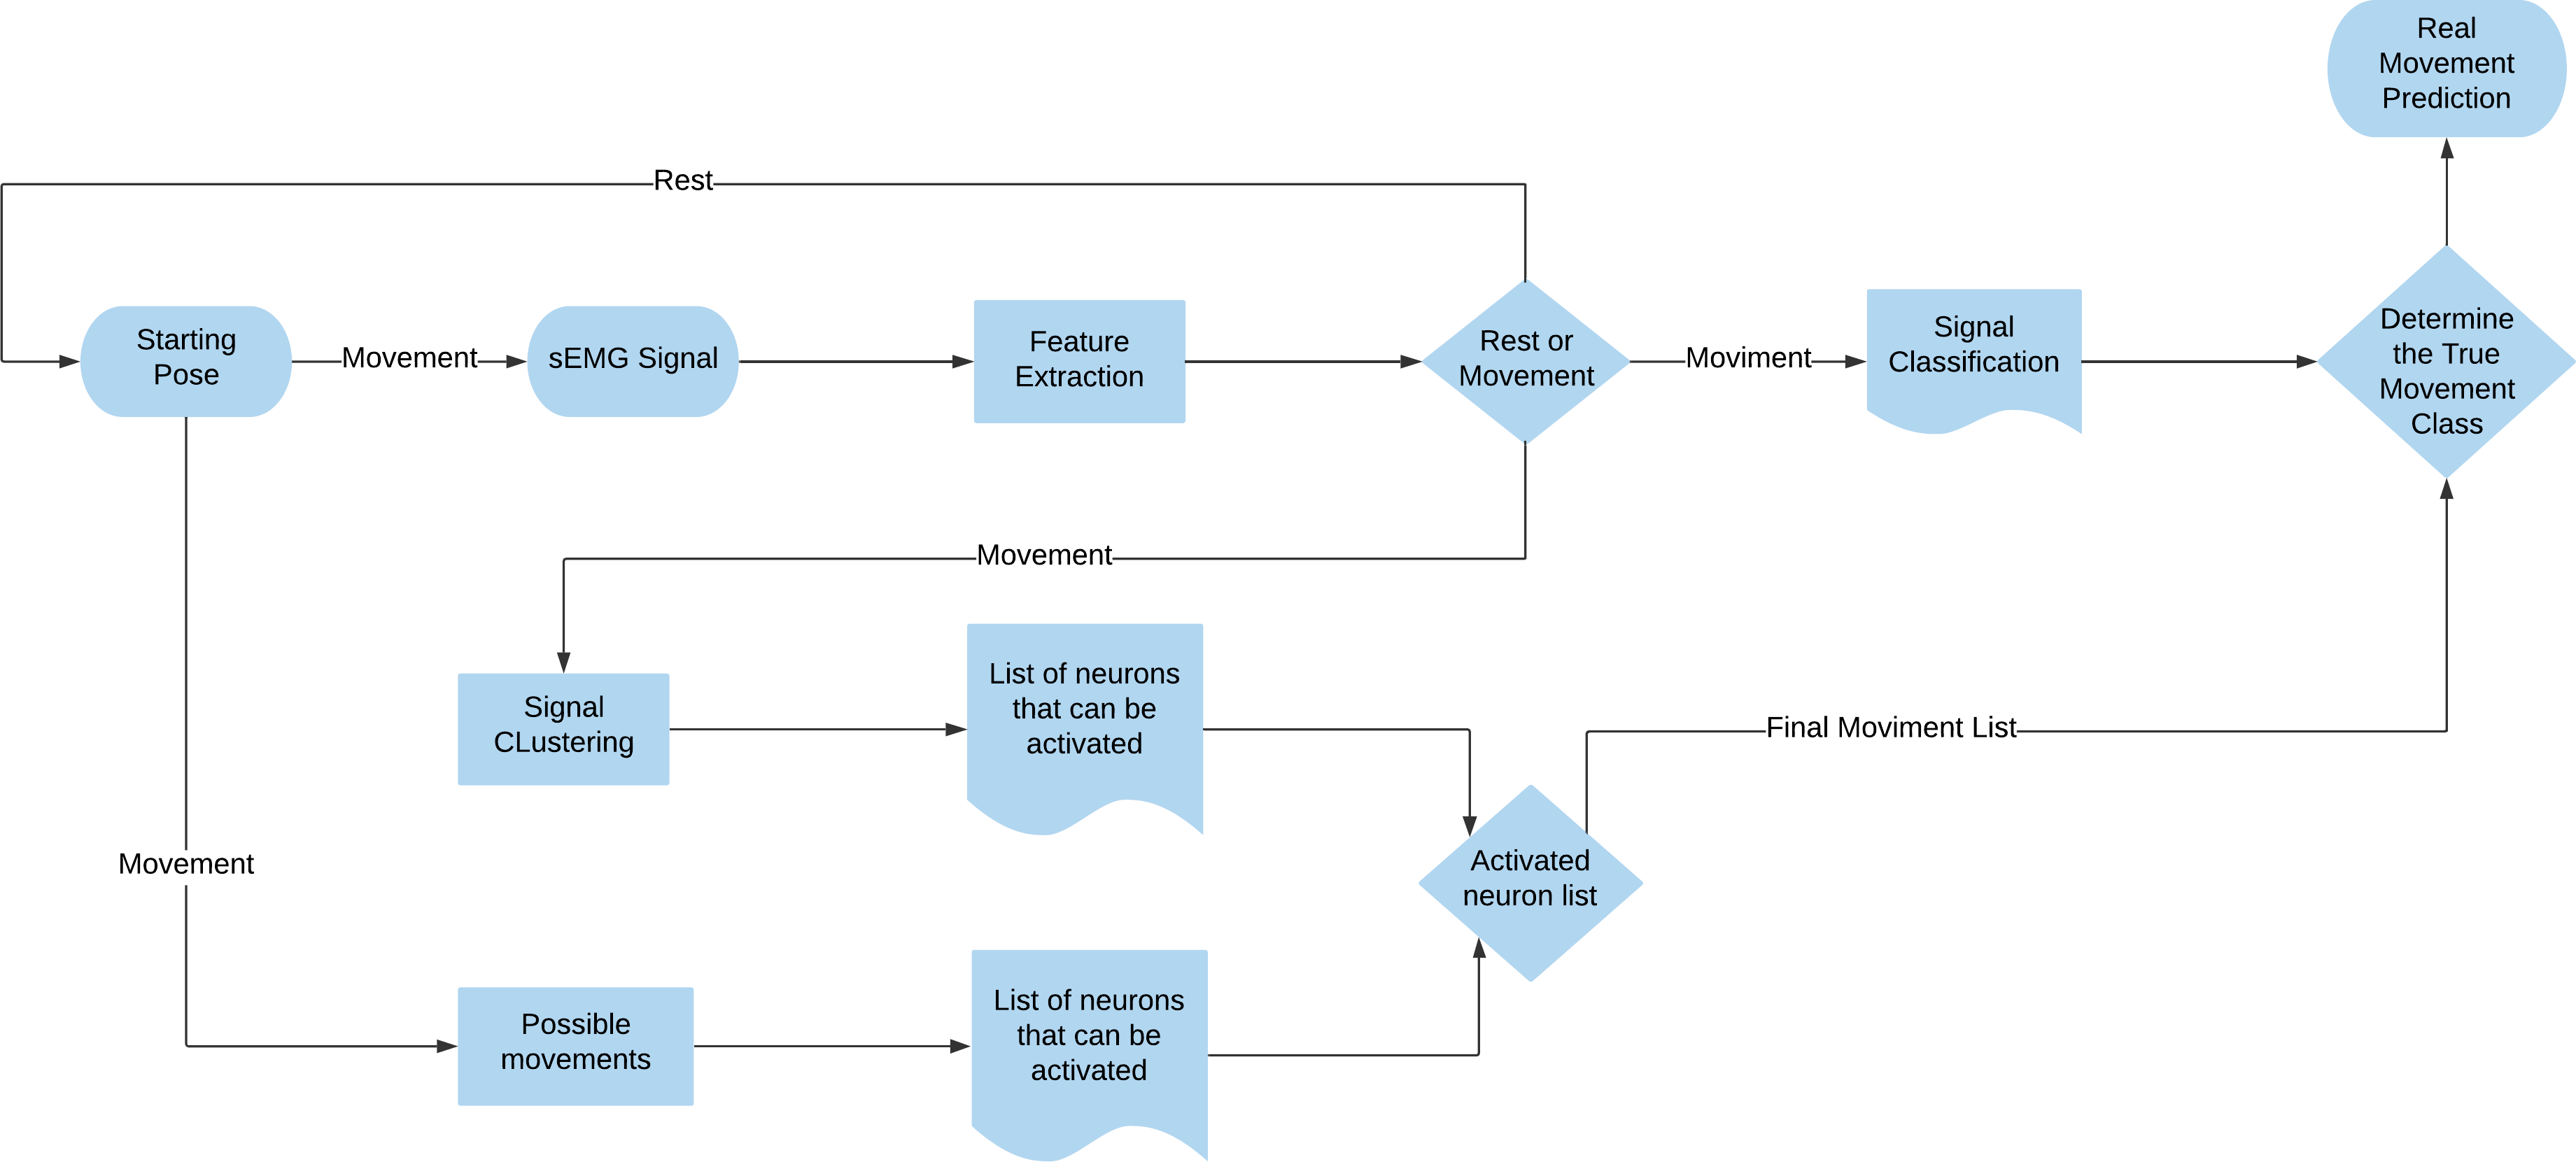
\includegraphics[width=.8\linewidth]{figuras/final_semg_classification.pdf}
%    \caption{Fluxograma utilizado para a classificação do sinal do sEMG}
%\end{figure}

\end{frame}

%%%%%%%%%%%

## Dataset
### Dataset

O banco de dados 6mov8chUFS, que está disponível na plataforma BioPatRec, foi usado. Esse banco de dados é formado por 17 sujeitos, foram selecionadas seis classes de movimentos individuais, como abertura e fechamento da mão, flexão e extensão do punho e pró-supinação da mão, formando 27 movimentos possíveis. O sinal foi medido da seguinte forma: 3 segundos de tempo de contração e 3 segundos para relaxamento entre cada repetição, repetições de cada movimento. 8 eletrodos bipolares (Ag / AgCl descartável), diâmetro de eletrodo de 1 cm, distância entre eletrodos de 2 cm para o bipolo. Os eletrodos foram igualmente espaçados em torno do terço mais proximal do antebraço.

\end{frame}

%%%%%%%%%%%
## Extração de Características
### Extração de Características

- The extracted characteristics are:
    - Spectral Moment (\ac{SM});
    - Sample Entropy (\ac{SE});
    - KhushabaSet;
    - Wave Lenght (WL) Frequency);
    - Mean Frequency;
    - Meadian Frequency.

\end{frame}

%%%%%%%%%%%
## Redução de Dimensionalidade
### Redução de Dimensionalidade

- Neighborhood Component Analysis (NCA)  [30]  permitiu a redução dimensional, ajudando a selecionar os recursos mais significativos do sinal. A NCA é um algoritmo de aprendizado supervisionado para aprendizado métrico à distância. Ele aprende uma transformação linear (de dados de entrada) que maximiza, no espaço transformado, o desempenho médio da classificação leave-one-out.


\end{frame}

%%%%%%%%%%%

### Teste de Algoritmos Redução de Dimensionalidade

\begin{figure}[h]
	\centering
	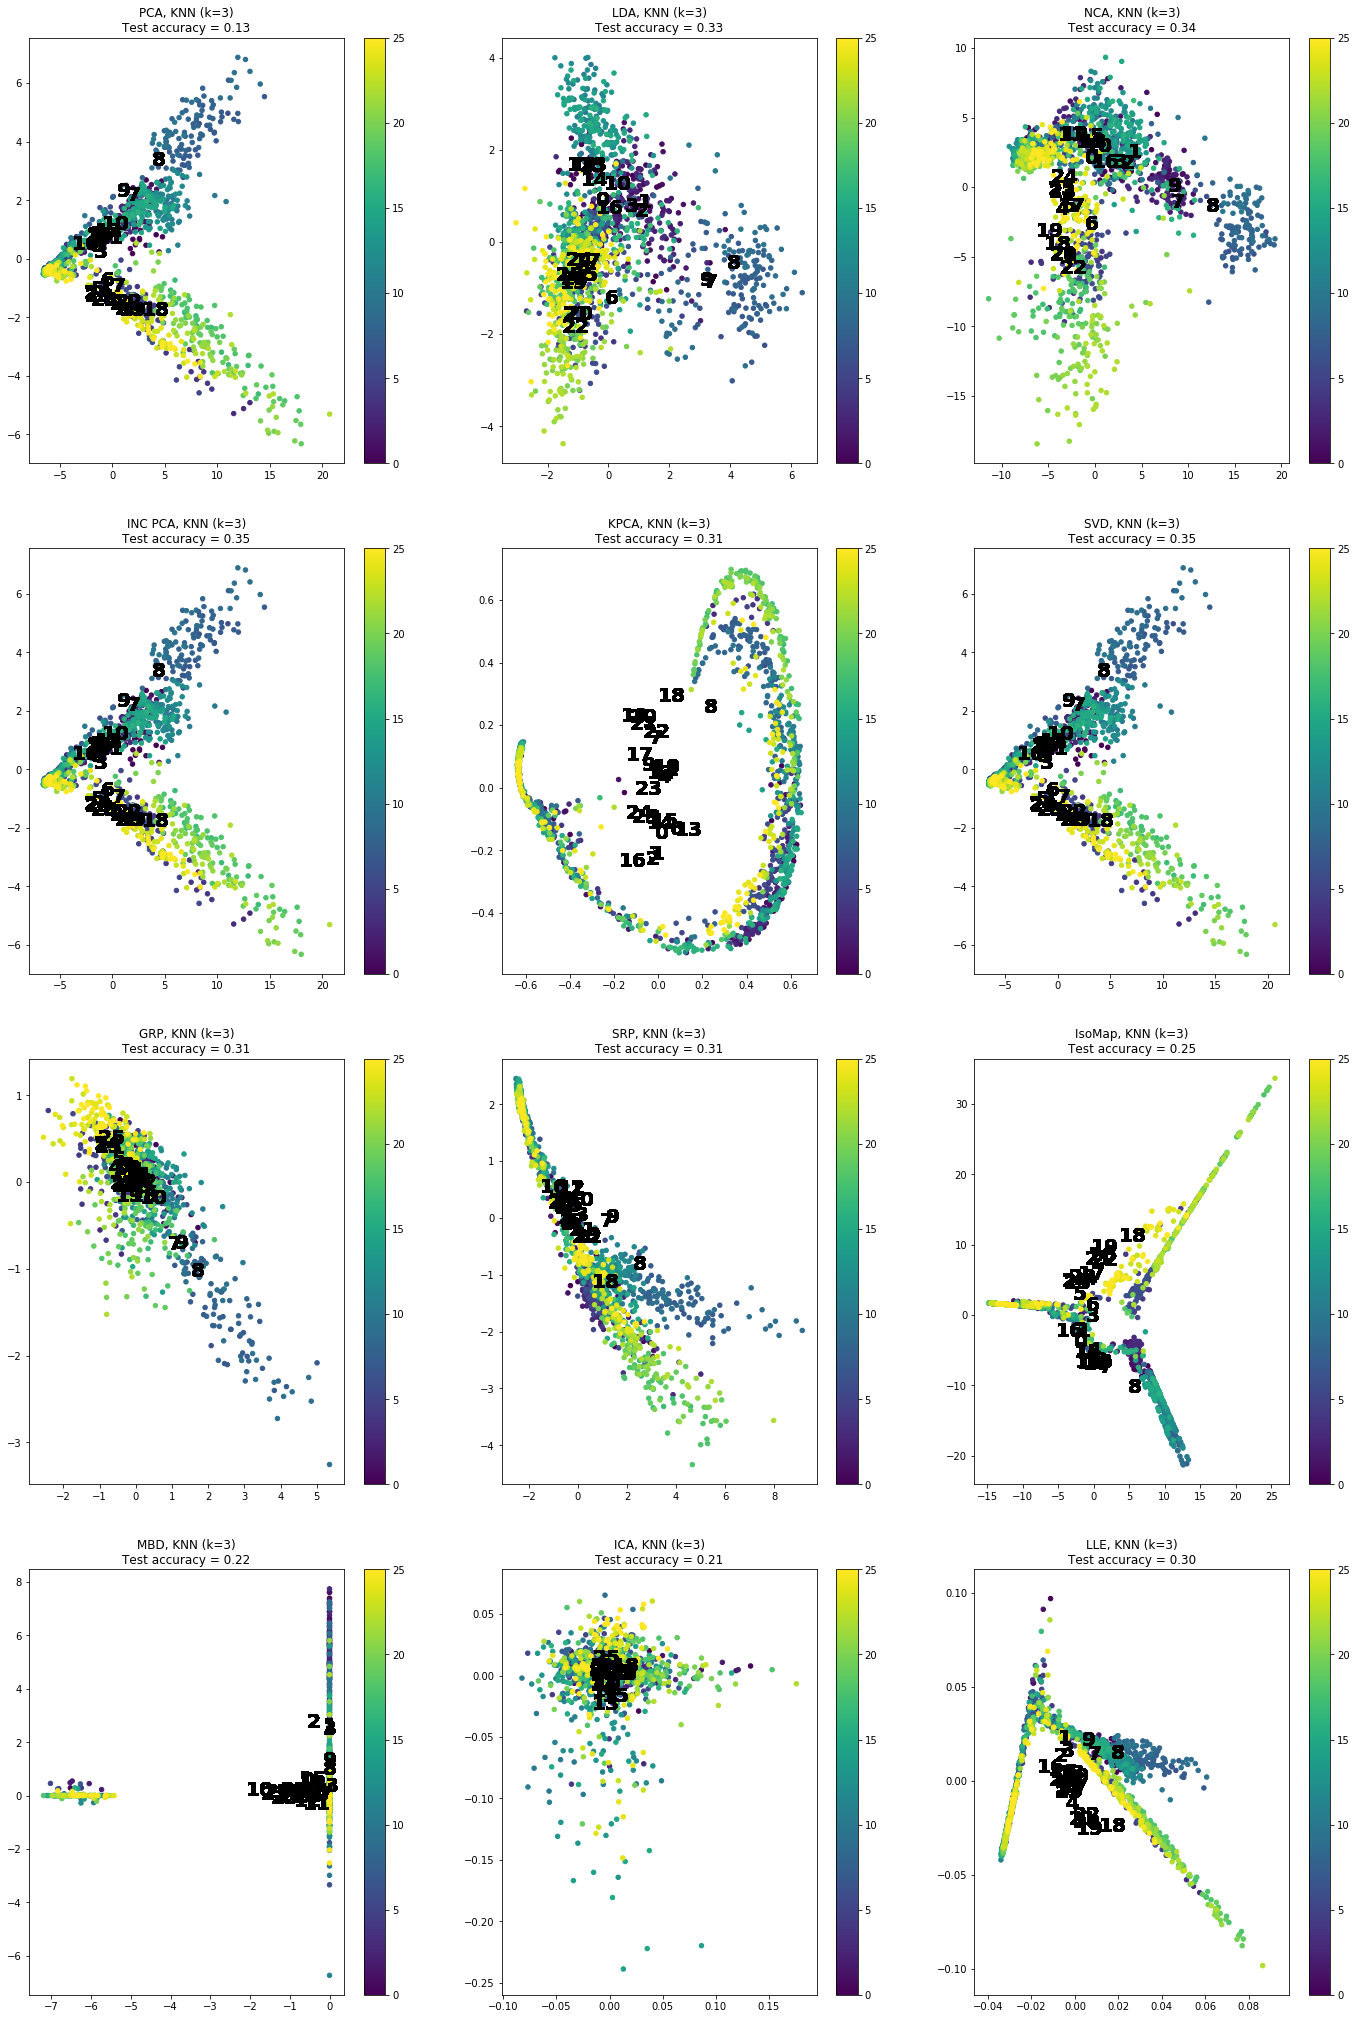
\includegraphics[width=.8\linewidth]{figuras/clustering_smg.png}
    \caption{Fluxograma utilizado para a classificação do sinal do sEMG}
\end{figure}

\end{frame}

%%%%%%%%%%%

## Detecção de Anomalia
### Detecção de Anomalia

Um autoencoder é uma rede neural treinada para tentar copiar sua entrada para sua saída. Embora a cópia da entrada para a saída possa ser inútil, um dado de alta dimensão pode ser convertido em códigos de baixa dimensão treinando uma rede neural multicamada com uma pequena camada central para reconstruir vetores de entrada de alta dimensão. Utilizando a camada interna, também chamada espaço latente, temos um sinal de tamanho reduzido, mais facilmente classificado.

\end{frame}

%%%%%%%%%%%

### Autoencoder Variacional

O Autoencodificador Variacional (VAE) é um tipo de autoencoder com um modelo generativo que estima a Função de Densidade de Probabilidade (PDF) dos dados de treinamento. Ao treinar o modelo para reconhecer o sinal sEMG, ele atribui um valor de alta probabilidade a uma classe de movimento, enquanto o ruído recebe um valor de baixa probabilidade

\end{frame}

%%%%%%%%%%%

### Visualização da Anomalia

%\begin{figure}[h]
%	\centering
%	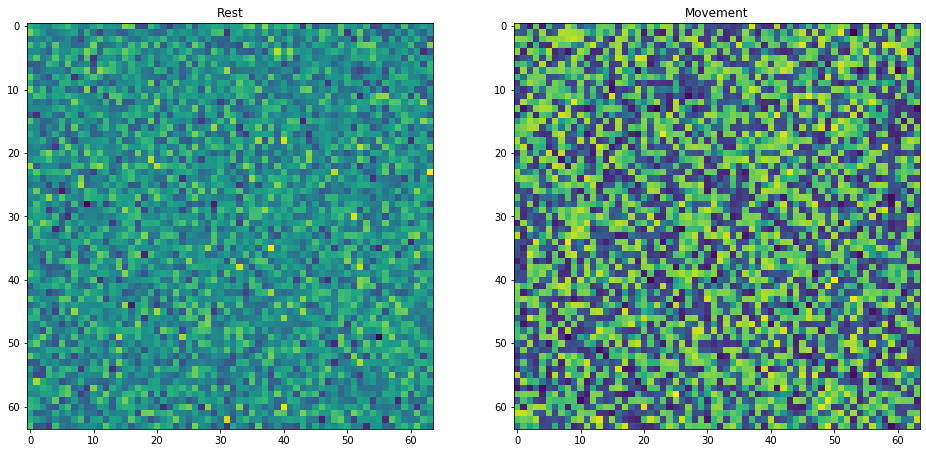
\includegraphics[width=.8\linewidth]{figuras/latent_space_as_image.png}
%    \caption{Fluxograma utilizado para a classificação do sinal do sEMG}
%\end{figure}

\end{frame}

%%%%%%%%%%%

## Classificação do Sinal
### Classificação do Sinal

%\begin{figure}[h]
%	\centering
%	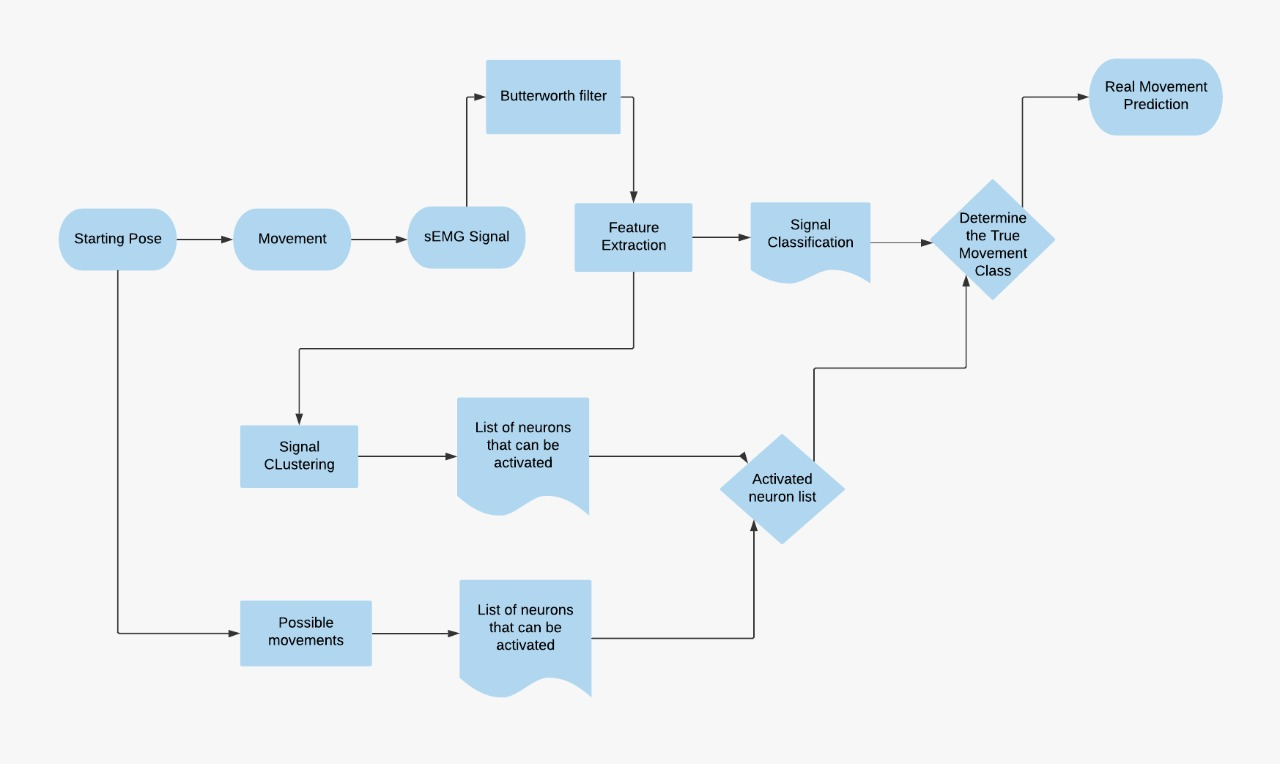
\includegraphics[width=.8\linewidth]{figuras/sMEG_Classification_Fluxogram.png}
%    \caption{Fluxograma utilizado para a classificação do sinal do sEMG}
%\end{figure}

\end{frame}

%%%%%%%%%%%

### Máquina de Estados

A partir de uma determinada posição do antebraço e mão é criada uma lista com os possíveis movimentos para o usuário.

\end{frame}

%%%%%%%%%%%

### Clustering

- Para o algoritmo de clustering aglomerativo hierárquico, que dividiu o sinal em três grupos de dados que foram avaliados usando KNN (k = 3). Esse KNN alcançou 97\% de precisão ao classificar os grupos. 

- Este método foi usado pois ele agrupa por similaridade. O algoritmo HAC coloca cada entrada como um cluster e em seguida mescla recursivamente pares de clusters de acordo com a distância entre eles.

\end{frame}

%%%%%%%%%%%

### Clustering

\begin{figure}[h]
	\centering
	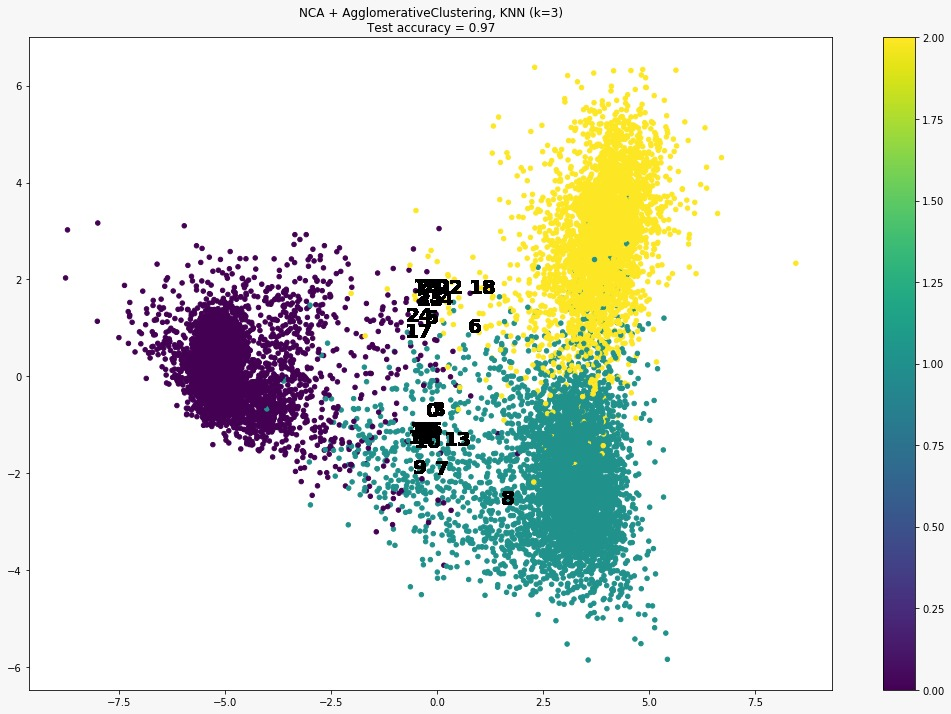
\includegraphics[width=.8\linewidth]{figuras/sMEG_Clustering.png}
    \caption{Clustering das classes pela similaridade nos recursos extraídos. Após a extração de vinte e cinco dimensões, as duas dimensões mais representativas entre elas foram utilizadas para gerar o gráfico}
\end{figure}

\end{frame}

%%%%%%%%%%%

### Classificação

%\begin{figure}[h]
%	\centering
%	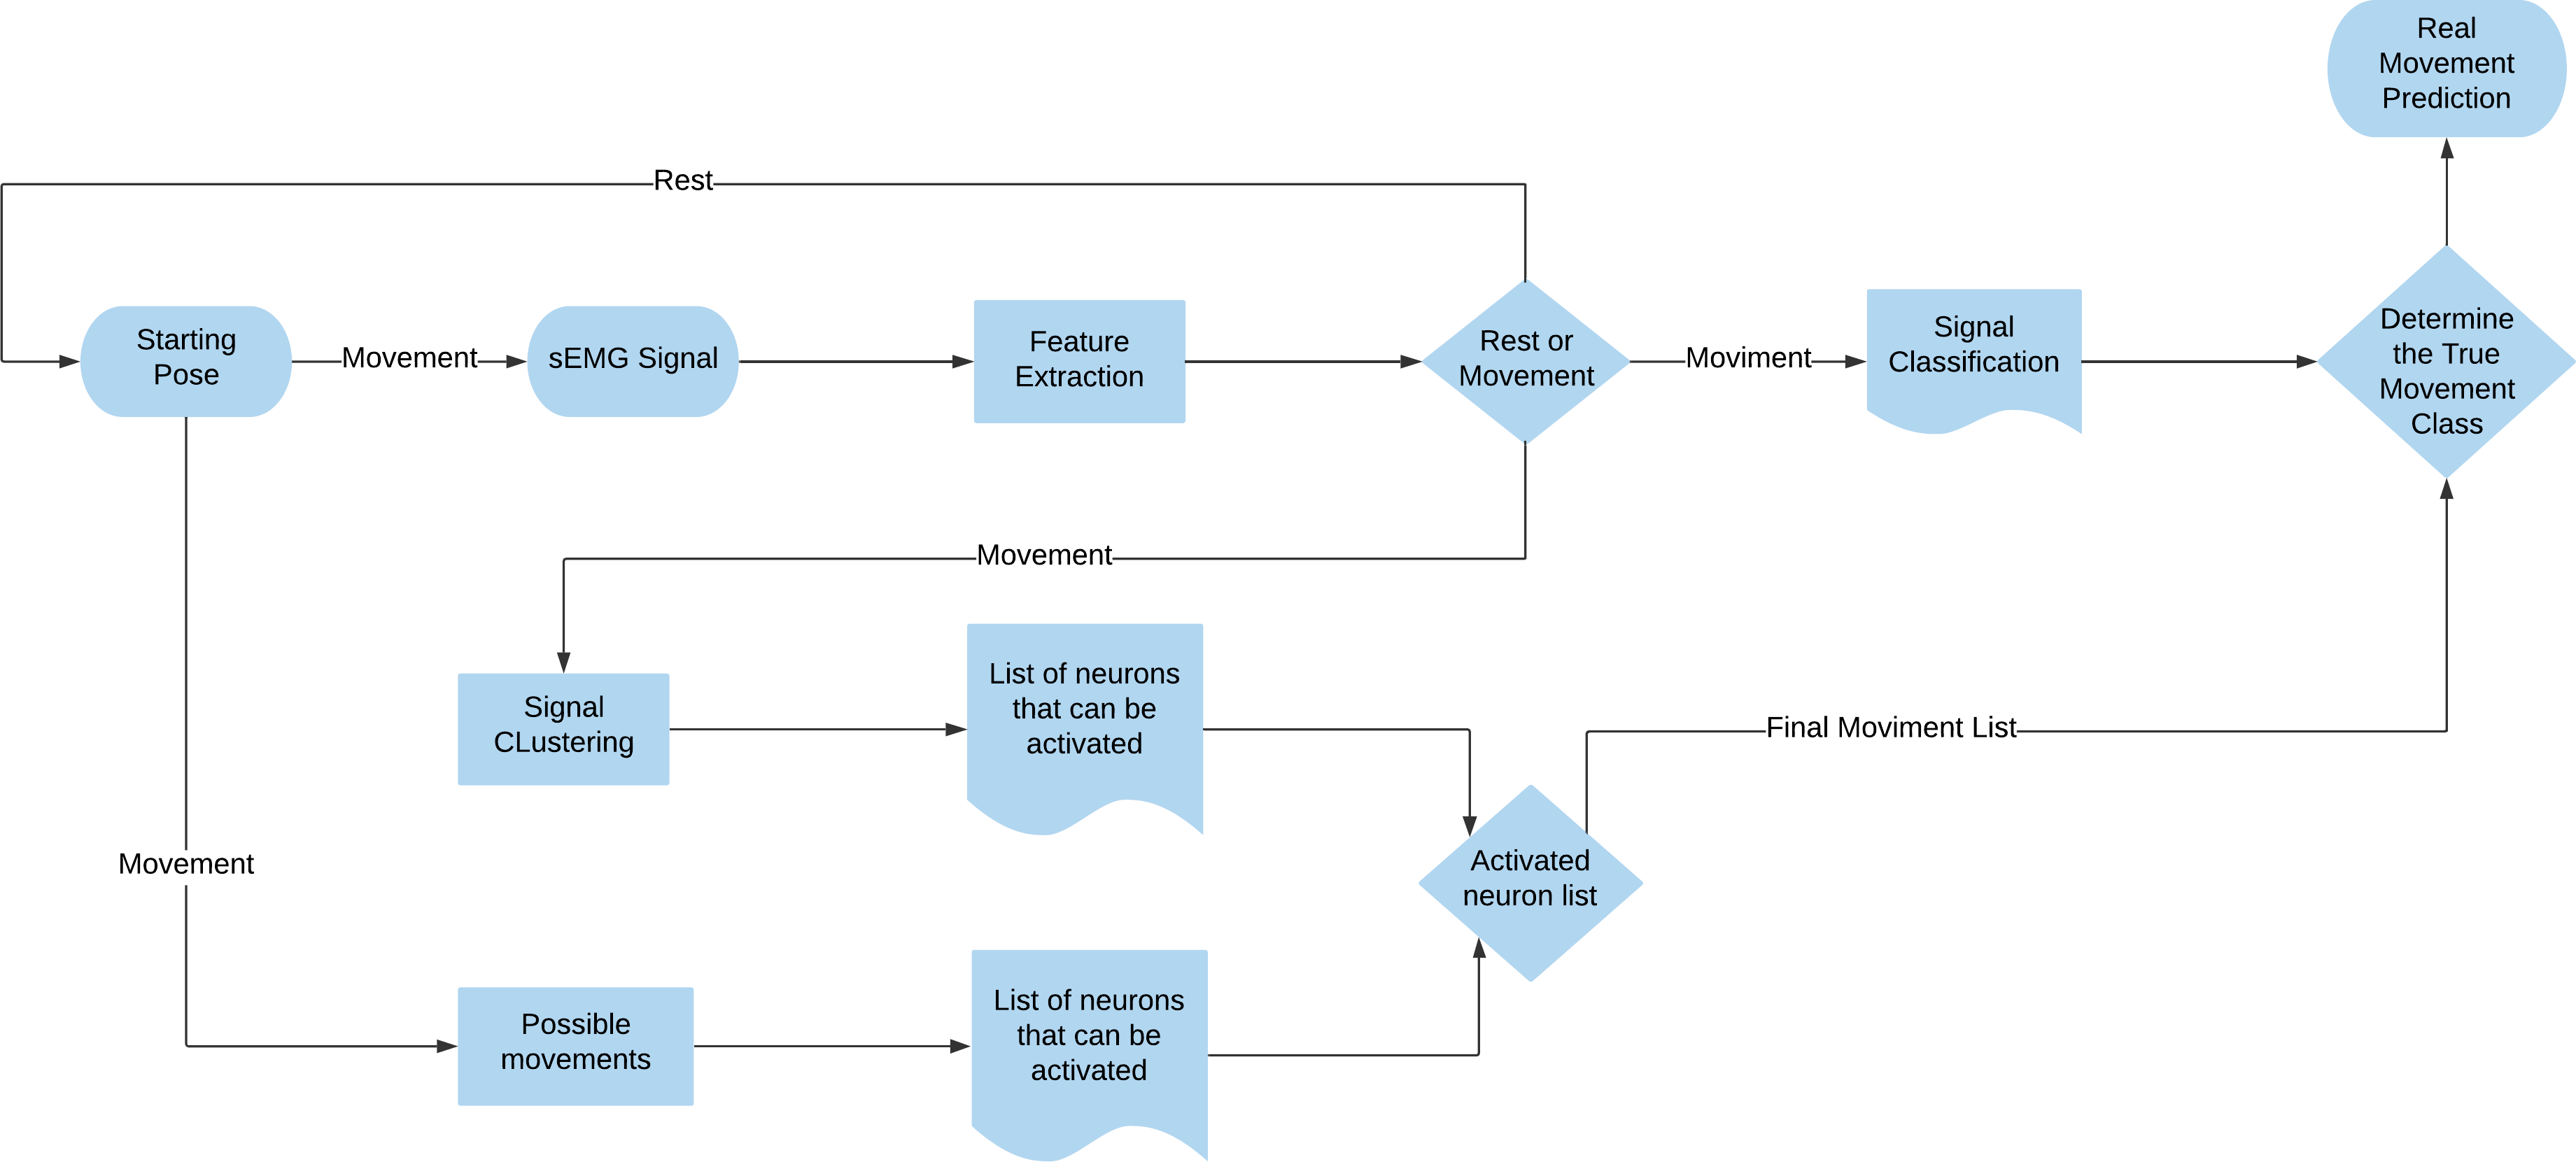
\includegraphics[width=.8\linewidth]{figuras/final_semg_classification.png}
%    \caption{Fluxograma utilizado para a classificação do sinal do sEMG}
%\end{figure}

\end{frame}

%%%%%%%%%%%

# Considerações Finais

### Considerações Finais

- Este estudo foi realizado com a intenção de levantar uma quantidade maior de informações sobre o sinal EMG.
- O processamento em tempo real foi considerado e modelos de inteligência artificial que suficientemente pequenos para serem executados em microcontroladores foram considerados como o principal problema desse estudo.
- Uma das dificuldades na classificação do sinal foi saber exatamente onde o movimento começou.


\end{frame}

%%%%%%%%%%%

### Considerações Finais

- O principal trabalho futuro seria a implementação do sistema e o teste com pacientes com aquisição ao vivo da EMGs.
- Novos métodos de redução da entropia antes do classificador devem ser testados. 
- Estudos adicionais devem ser realizados para encontrar novas formas de diminuir a entropia do sinal antes de sua classificação final.


\end{frame}

%%%%%%%%%%%

%### Pipe Tables
%
%- Use `pipeTables` and `tableCaptions` options
%- Available since `markdown` v2.8.0
%
%| Right | Left | Default | Center |
%|------:|:-----|---------|:------:| 
%|  12   |  12  |  12     |   12   | 
%| 123   |  123 |   123   |  123   | 
%|   1   |    1 |     1   |    1   | 

%  : Demonstration of pipe table syntax.
  
%\end{frame}

%%novalidate
\end{markdown}

\begin{frame}
\renewcommand{\bibfont}{\footnotesize}
\frametitle{Bibliography}

\bibliographystyle{apalike}
\bibliography{refs}

\end{frame}

%%%%%%%%%%%

\maketitle

%%%%%%%%%%%

\end{document}
